\subsection{Second Experience}

\subsubsection{Python UDP Implementation (Loopback)}

After setting up a Python environment and running both scripts, we got the
following output:

\begin{figure}[htbp]
	\centering
	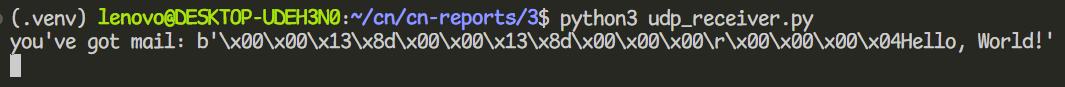
\includegraphics[width=1\linewidth]{img/second_exp/1.png}
	\caption{Receiver Output}\label{fig:2_1}
\end{figure}

\begin{figure}[htbp]
	\centering
	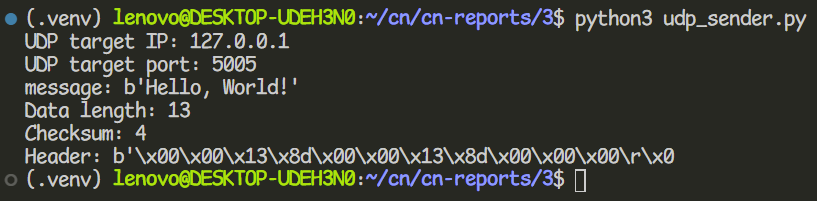
\includegraphics[width=1\linewidth]{img/second_exp/2.png}
	\caption{Sender Output}\label{fig:2_2}
\end{figure}

We can see that the received header matches the data sent by the sender, and
the IP is 127.0.0.1 as we were listening to that specific ip-port combination.

To further analyze the UDP package, we opened Wireshark and looked for the UDP
package.

\begin{figure}[htbp]
	\centering
	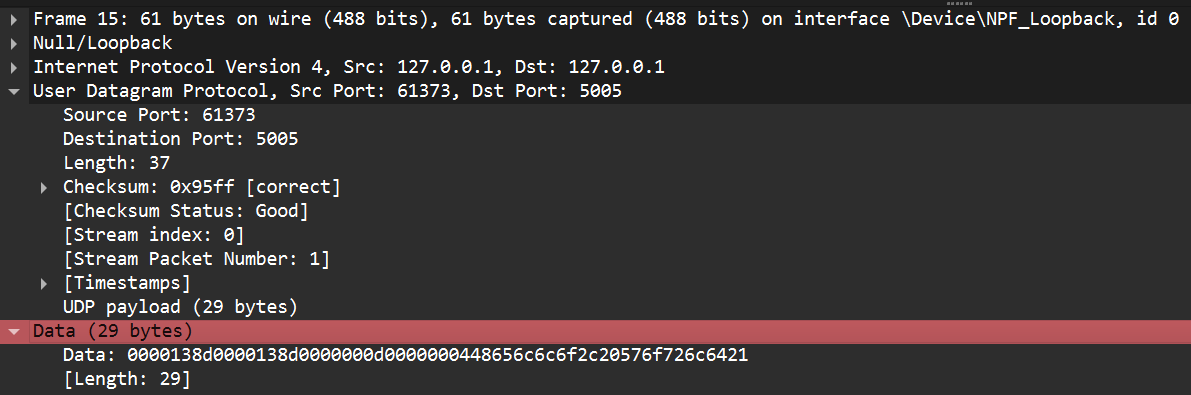
\includegraphics[width=1\linewidth]{img/second_exp/3.png}
	\caption{}\label{fig:2_3}
\end{figure}

The source port is 61373, which can be interpreted as a private port.
Destination port is 5005.

To send the UDP packet to a different PC, we would need to

\begin{itemize}
	\item be on the same network
	\item open port 5005 on the receiver PC (firewall might mess it up)
	\item change the target ip address in the python file
\end{itemize}

We also wanted to compare checksum values, and analyzed a different packet for
such task.

\begin{figure}[htbp]
	\centering
	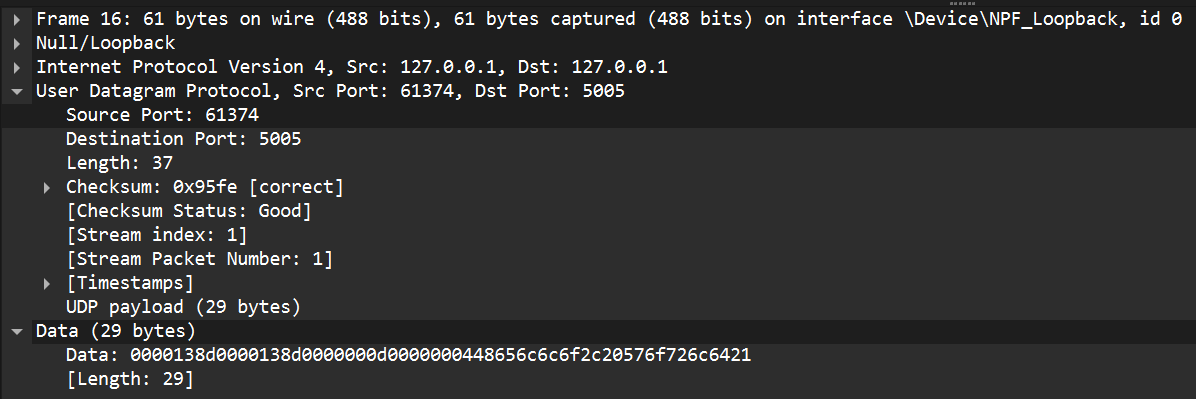
\includegraphics[width=1\linewidth]{img/second_exp/4.png}
	\caption{}\label{fig:2_4}
\end{figure}

The checksum is different by one bit. The checksum was calculated and validated
correctly, as displayed by Wireshark.

The 128 TTL value is set by Windows for outgoing IP packets, and as it never
leaves the PC, its TTL never changes (no hostname resolution).

The Wireshark packet is identified as UDP, as it assumes it is UDP by the port
number. According to a short research, it might also use heuristics if port
doesn't match a known protocol.

\subsubsection{Python UDP Implementation (P2P)}